\documentclass[a4paper,11pt,dvipdfmx]{jsarticle}

\usepackage{latexsym,amsmath,amssymb} % 数式関連. とりあえず入れとく 
\usepackage{graphicx} % includegraphics に必要
\usepackage{ascmac}
\usepackage{amsmath}
\usepackage{latexsym}



\title{{\LaTeX}演習資料}
\author{離散太郎}
\date{京都大学\\E-mail: risan@risan-suuri.org}
% \author{京都大学}
% \author{E-mail: risan@risan_suuri.org}


\begin{document}

\maketitle

\section{はじめに}
個人から集団に至るまで, 日々の活動では直面した問題に対する計画や意思決定の作業が不可欠 である. 
ところが現実の問題は曖昧模糊としており, 何を基準に判断を下せばいいのかもよくわか らないことが多い. 

問題を\textbf{数理} ー数の持つ理ー 的な視点から解決できないだろうか. 
数理的な手法を用いた問題解 決について研究を重ねてきた学問領域が, \textbf{オペレーションズ・リサーチ} (operations research, OR と略される) である. 
OR では一般的な問題解決の流れとして,

\begin{enumerate}
\item 現実の問題を\textbf{数理モデル}として\textbf{定式化} (formulation)し, 
\item 計算によってその解を求め
\item 結果を元の問題の解決に役立てる
\end{enumerate}

という手続きがとられる. ただしこの手続きは決定的なものではない. 
1 回行なえば十分というも のではなく, 満足な解決策を得るためには何度も反復しなければならないかもしれない. 
また\textbf{2}の結果に基づいて\textbf{1}を再検討するなど, 必ずしも\textbf{1 → 2 → 3}の順で行なわれるわけではない.

いずれにせよ, 定式化のための数理モデルと, それを解くための\textbf{アルゴリズム} (algorithm, 計算 の手順) が必要となろう. 
\textbf{数理最適化} (mathematical optimization) は代表的な数理モデルの 1つだが, 以下では数理最適化問題とはどのような問題かを示し, 線形最適化, 整数最適化, 組合せ最適化の概要を示す.

\subsection{数理最適化問題}
\textbf{数理最適化問題} (mathematical optimization problem), あるいは単純に\textbf{最適化問題} (optimiza- tion problem) とは, 
与えられた\textbf{目的関数} (objective function) と\textbf{制約条件} (constraints) に対し, 制約条件を満たす\textbf{解} (solution) のうち, 
目的関数の値が最大 (あるいは最小) となるものを問う問題である. 
目的関数を $f$, 制約条件を満たす解すべての集合を $F$ と書くことにすると, 最適化問題の一般系は以下のように表される. 

\begin{shadebox}
    \begin{alignat*}{2}
    &\textbf{maximize} \quad &f(x)   \\
    &\text{(あるいは}\textbf{minimize})&  \\
    &\textbf{subject to} &x \in F 
    \end{alignat*}
\end{shadebox}

制約条件を満たす解を\textbf{実行可能解} (feasible solution) といい\footnote{\textbf{許容解} (admissible solution)ともいう. }, その集合$F$を\textbf{実行可能領域} (feasible region) という.

高校数学に出てくる次のような問題は, 最適化問題とみなすことができる.

2次関数 $y$ について, $y$の最小値, およびそれを達成する$x$の値を求めよ. 

\centerline{ただし $0 \leq x \leq 3$とする.}

\begin{screen}
    \begin{alignat*}{2}
    &\textbf{minimize}& \qquad & x^2-2x+4 \\
    &\textbf{subject to}& \qquad & 0\leq x \leq 3
    \end{alignat*}
\end{screen}
最適化問題は, 目的関数$f$や実行可能領域$F$がどのように表現されるか, あるいはどのような 特徴を持つかに応じていくつかのサブクラスに分類される.

\subsection{線形最適化問題}
最適化問題のサブクラスのうち最も基本的な問題が, \textbf{線形最適化問題} (linear optimization problem) である\footnote{この問題は約半世紀にわたって線形計画問題 (linear programming problem, LP) と呼ばれてきたが, 
現在は線形最適化問題と呼ばれるのが主流である. }. 
線形最適化問題とは, 解が実数変数のベクトル $(x_1, x_2, . . . , x_n)$ によって表され, 目的関数が変数に関する1次関数, 
制約条件が変数に関する 1 次の等式または不等式の集合で 与えられるような最適化問題である.

\begin{shadebox}
    \centering
    \begin{tabular}{l c r c r c r c c l l l}
        \textbf{maximize}   &  & $3x_1$ & $+$ & $4x_2$ & +              & $2x_3$             &      &   &  &  &  \\
        \textbf{subject to} &  & $2x_1$ &     &        &                &                    & $\leq$ & $4$ &  &  &  \\
                            &  & $x_1$  &     &        & +              & $2x_3$             & $\leq$ & $8$ &  &  &  \\
                            &  &        &     & $3x_2$ & +              & $x_3$              & $\leq$ & $6$ &  &  &  \\
                            &  &        &     &        & \multicolumn{2}{l}{$x_1, x_2, x_3$} & $\leq$ & $0$ &  &  & 
    \end{tabular}
    % \end{table}
\end{shadebox}

\subsection{整数最適化問題}
解が変数のベクトル $(x_1,x_2,...,x_n)$ によって表されるが, 変数のすべて, あるいは一部が, 整数値を取らなければならないという制約が課された最適化問題を\textbf{整数最適化問題} (integer optimization problem) という\footnote{ LP 同様, これも整数計画問題 (integer programming problem, IP) と呼ばれてきた.}. 
特に, 線形最適化問題同様, 目的関数が変数に関する 1 次関数, 制約条件が変数に関する 1 次の等式または不等式の集合で与えられるような整数最適化問題を\textbf{整数線形最適化問題} (integer linear optimization problem) という.
\begin{shadebox}
    \centering
    \begin{tabular}{l c r c r c r c c l l l}
        \textbf{maximize}   &  & $3x_1$ & $+$ & $4x_2$ & +              & $2x_3$             &      &   &  &  &  \\
        \textbf{subject to} &  & $2x_1$ &     &        &                &                    & $\leq$ & $4$ &  &  &  \\
                            &  & $x_1$  &     &        & +              & $2x_3$             & $\leq$ & $8$ &  &  &  \\
                            &  &        &     & $3x_2$ & +              & $x_3$              & $\leq$ & $6$ &  &  &  \\
                            &  &        &     &        & \multicolumn{2}{l}{$x_1, x_2, x_3$} & $\leq$ & $0$ &  &  & \\
                            &&&&&&\multicolumn{3}{l}{\underline{$x_1,x_2$は整数}}&&&
    \end{tabular}
\end{shadebox}

\subsection{組合せ最適化問題}
最適化問題のうち, 解が「組合せ的構造」を持つものを組合せ最適化問題 (combinatorial optimization problem) という\footnote{\textbf{離散最適化問題}(discrete optimization problem) ともいう.}. 
何をもって「組合せ的」と呼ぶか, その定義は簡単ではないが, たとえば2値ベクトル (各要素は 0 もしくは 1 のいずれかを取る) で解が表される問題や, 順列や集合によって解が表される問題は組合せ最適化問題として取り扱われることが多い.

組合せ最適化問題とそうでない問題の間に, 明確な区別がなされているわけではない. たとえば 線形最適化問題は, 解が実数変数のベクトルで表されるという点では組合せ的ではないが, 問題が 持つある特徴により, 組合せ最適化問題として取り扱われることが多い.

現実に応用を持つ様々な組合せ最適化問題が知られているが, そのうちいくつかを以下に紹介 する.

$\blacksquare$ \textbf{巡回セールスマン問題}
\begin{shadebox}
    $n$個の都市があり, 任意の2つの都市の間について, 移動に要する時間が与えられている. 
    任意の都市を出発し, ほかのすべての都市をちょうど 1 度ずつ訪れて最初の都市に戻る巡回路 のうち, 合計時間が最小となるようなものを求めよ.
\end{shadebox}
この問題はその名前から応用がすぐに思い浮かぶが, 配送計画, プリント基盤の作成やDNA解析などにも応用を持つ. \\

$\blacksquare$ \textbf{最大クリーク問題} 
\quad 単純な無向グラフにおいて, 極大な完全部分グラフを\textbf{クリーク}という. 
たとえば図1のグラフにおいて, $\{a, b, d, e\}$, $\{b, c, e\}$ はクリークだが, $\{a, b, e\}$ はクリークでない (極大でないから).

\begin{figure}[htbp]
    \begin{center}
    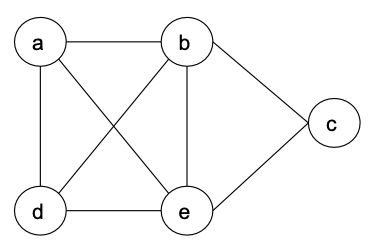
\includegraphics[width=50mm]{0519_kr}
    \caption{単純な無向グラフ}
    \end{center}
\end{figure}

\begin{shadebox}
与えられたグラフにおける最大サイズのクリークを求めよ.    
\end{shadebox}
この問題は, 例えばSNSのコミュニティ発見など, ネットワーク解析に応用を持つ問題である. 


\end{document}

